%!TEX root = ../template.tex
%%%%%%%%%%%%%%%%%%%%%%%%%%%%%%%%%%%%%%%%%%%%%%%%%%%%%%%%%%%%%%%%%%%%
%% chapter3.tex
%% NOVA thesis document file
%%
%% Chapter with a short latex tutorial and examples
%%%%%%%%%%%%%%%%%%%%%%%%%%%%%%%%%%%%%%%%%%%%%%%%%%%%%%%%%%%%%%%%%%%%

\typeout{NT FILE chapter3.tex}%

\makeatletter
\newcommand{\ntifpkgloaded}{%
  \@ifpackageloaded%
}
\makeatother


\chapter{Experiment}
\label{cha:experiment}

\epigraph{
	"Somewhere, something incredible is waiting to be known."
}{Carl Sagan}



\section{Context and Goal of the Experiment} % (fold)
\label{sec:contex_goal_experiment}

The proposed experiment, detailed in research proposal G-24-00249, aims to investigate the structure of the neutron-rich fluorine isotope, $^{25}$F, through one-proton knockout reactions. This study is motivated by the "drastic extension of the neutron drip line for Z=9 compared to Z=8 isotopes," a phenomenon that remains poorly understood (Ahn et al., 2019). The experiment seeks to elucidate how the $^{24}$O core is polarized by the presence of an additional proton in $^{25}$F, thereby shedding light on the mechanisms responsible for the observed drip line extension.

The experiment will employ the quasi-free scattering (QFS) reaction $^{25}$F(p,2p)$^{24}$O in inverse kinematics, effectively knocking out a deeply bound valence proton from the $^{25}$F nucleus (Panin et al., 2016). This approach will utilize the R3B experimental setup, including the high-efficiency neutron detector NeuLAND, to achieve complete kinematic measurements and obtain accurate spectroscopic information on the populated final states of $^{24}$O (Boretzky et al., 2021). By analyzing the experimental data, researchers aim to determine the extent to which the single d5/2 proton in $^{25}$F modifies the structure of the core nucleons, potentially indicating deformation or polarization of the $^{24}$O core (Macchiavelli et al., 2020).

Ultimately, the goal of this experiment is to provide a more detailed understanding of the nuclear structure of neutron-rich fluorine isotopes and the underlying reasons for the extended neutron drip line at Z=9. The results will contribute to a more comprehensive picture of nuclear forces and structure in exotic nuclei, addressing a fundamental question in nuclear physics.


\section{The GSI Accelerator System}


\section{R3B Setup}

\gls{R3B}


\begin{figure}
	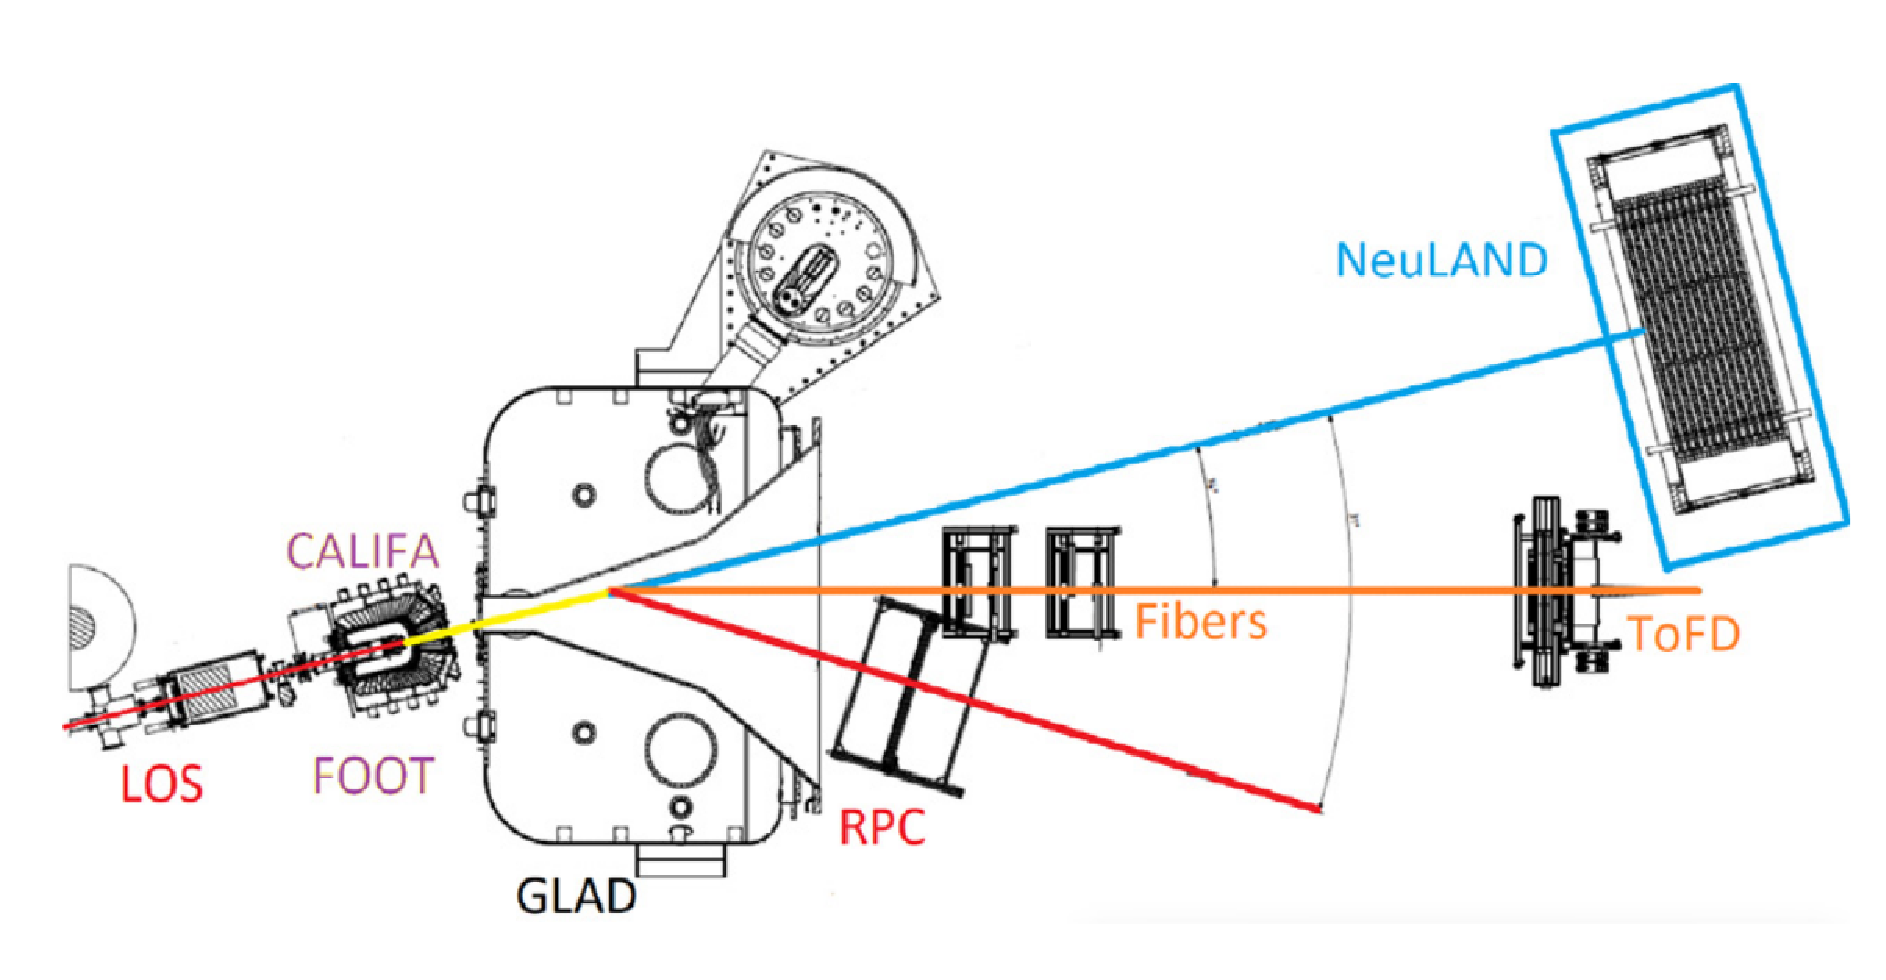
\includegraphics[width=\linewidth]{SchematicR3BSetup}
	\caption{Schematic representation of the R3B setup.}
	\label{fig:R3BSetup}
\end{figure}


\subsection{Role of each detector}



\subsection{Particular Role of RPC}



\section{Personal Contribution to the Experiment}